\documentclass{standalone}
\usepackage{tikz}
\usetikzlibrary{patterns, positioning}


\begin{document}
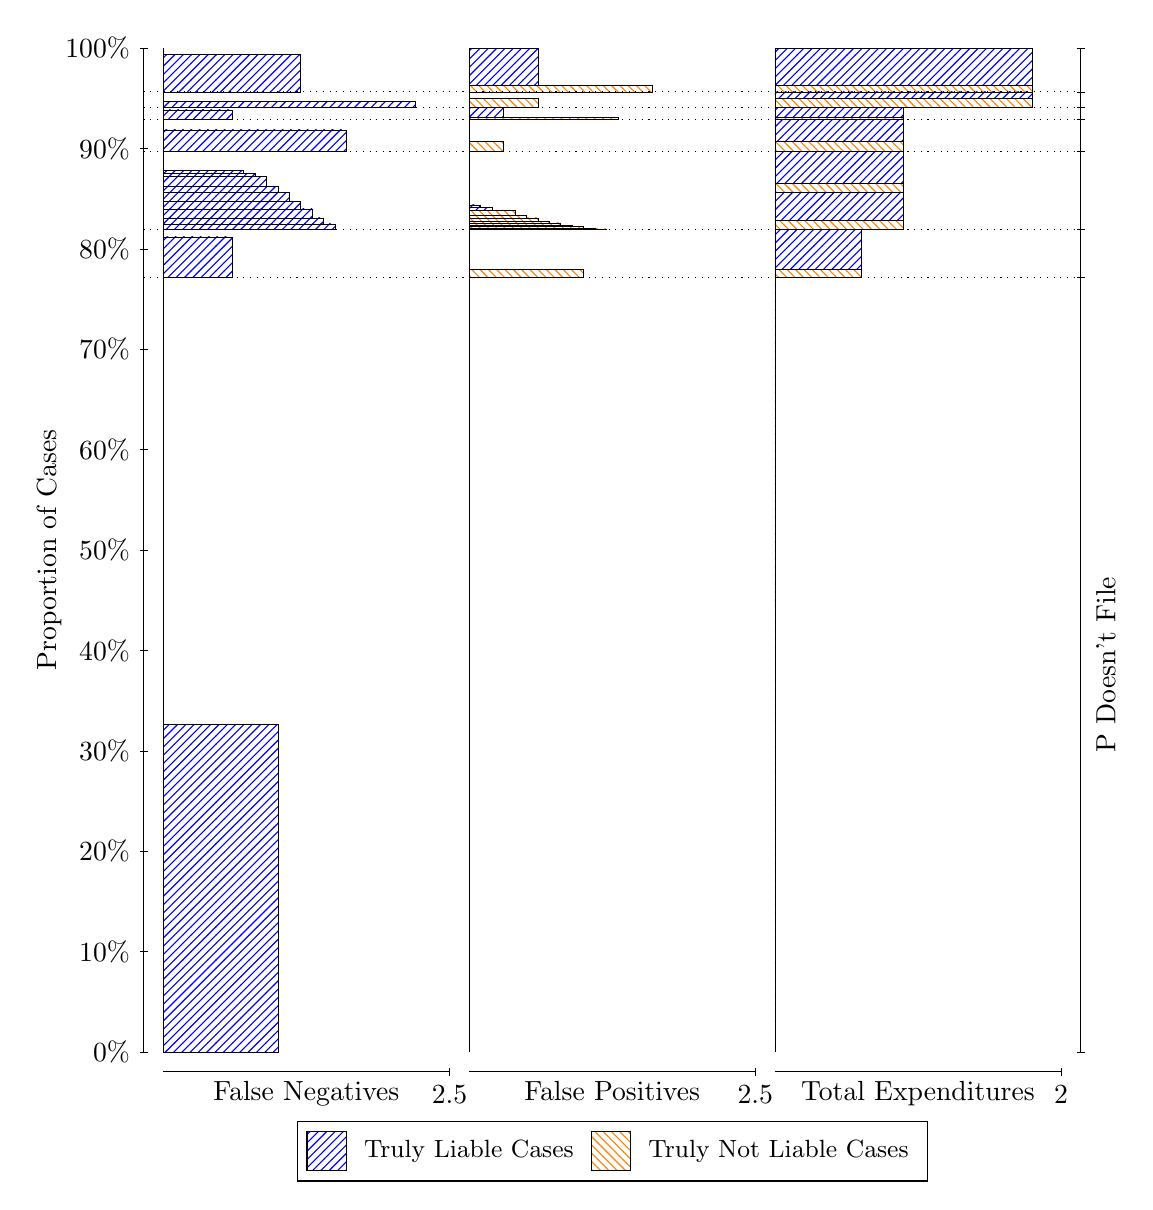
\begin{tikzpicture}
\draw[black, very thin] (1.5,1.75) -- (1.5,14.5);
\node[rotate=90, text=black, anchor=center] at (0.3, 8.125) {Proportion of Cases};
\draw[black, very thin] (1.45,1.75) -- (1.55,1.75);
\node[text=black, anchor=east] at (1.45, 1.75) {0\%};
\draw[black, very thin] (1.45,3.025) -- (1.55,3.025);
\node[text=black, anchor=east] at (1.45, 3.025) {10\%};
\draw[black, very thin] (1.45,4.3) -- (1.55,4.3);
\node[text=black, anchor=east] at (1.45, 4.3) {20\%};
\draw[black, very thin] (1.45,5.575) -- (1.55,5.575);
\node[text=black, anchor=east] at (1.45, 5.575) {30\%};
\draw[black, very thin] (1.45,6.85) -- (1.55,6.85);
\node[text=black, anchor=east] at (1.45, 6.85) {40\%};
\draw[black, very thin] (1.45,8.125) -- (1.55,8.125);
\node[text=black, anchor=east] at (1.45, 8.125) {50\%};
\draw[black, very thin] (1.45,9.4) -- (1.55,9.4);
\node[text=black, anchor=east] at (1.45, 9.4) {60\%};
\draw[black, very thin] (1.45,10.675) -- (1.55,10.675);
\node[text=black, anchor=east] at (1.45, 10.675) {70\%};
\draw[black, very thin] (1.45,11.95) -- (1.55,11.95);
\node[text=black, anchor=east] at (1.45, 11.95) {80\%};
\draw[black, very thin] (1.45,13.225) -- (1.55,13.225);
\node[text=black, anchor=east] at (1.45, 13.225) {90\%};
\draw[black, very thin] (1.45,14.5) -- (1.55,14.5);
\node[text=black, anchor=east] at (1.45, 14.5) {100\%};

\draw[black, very thin] (13.4,1.75) -- (13.4,14.5);
\draw[black, very thin] (13.35,1.75) -- (13.45,1.75);
\node[anchor=west] at (13.35, 1.75) {};
\draw[black, very thin] (13.35,11.588) -- (13.45,11.588);
\node[anchor=west] at (13.35, 11.588) {};
\draw[black, very thin] (13.35,12.196) -- (13.45,12.196);
\node[anchor=west] at (13.35, 12.196) {};
\draw[black, very thin] (13.35,13.184) -- (13.45,13.184);
\node[anchor=west] at (13.35, 13.184) {};
\draw[black, very thin] (13.35,13.596) -- (13.45,13.596);
\node[anchor=west] at (13.35, 13.596) {};
\draw[black, very thin] (13.35,13.743) -- (13.45,13.743);
\node[anchor=west] at (13.35, 13.743) {};
\draw[black, very thin] (13.35,13.943) -- (13.45,13.943);
\node[anchor=west] at (13.35, 13.943) {};
\draw[black, very thin] (13.35,14.5) -- (13.45,14.5);
\node[anchor=west] at (13.35, 14.5) {};

\draw[black, very thin, pattern color=blue, pattern=north east lines] (1.75,1.75) rectangle (3.2033,5.9133);
\draw[black, very thin, pattern color=orange, pattern=north west lines] (1.75,5.9133) rectangle (1.75,11.588);
\draw[black, very thin, pattern color=blue, pattern=north east lines] (1.75,11.588) rectangle (2.622,12.101);
\draw[black, very thin, pattern color=orange, pattern=north west lines] (1.75,12.101) rectangle (1.75,12.196);
\draw[black, very thin, pattern color=blue, pattern=north east lines] (1.75,12.196) rectangle (3.93,12.266);
\draw[black, very thin, pattern color=blue, pattern=north east lines] (1.75,12.266) rectangle (3.7847,12.343);
\draw[black, very thin, pattern color=blue, pattern=north east lines] (1.75,12.343) rectangle (3.6393,12.457);
\draw[black, very thin, pattern color=blue, pattern=north east lines] (1.75,12.457) rectangle (3.494,12.554);
\draw[black, very thin, pattern color=blue, pattern=north east lines] (1.75,12.554) rectangle (3.3487,12.668);
\draw[black, very thin, pattern color=blue, pattern=north east lines] (1.75,12.668) rectangle (3.2033,12.743);
\draw[black, very thin, pattern color=blue, pattern=north east lines] (1.75,12.743) rectangle (3.058,12.871);
\draw[black, very thin, pattern color=blue, pattern=north east lines] (1.75,12.871) rectangle (2.9127,12.908);
\draw[black, very thin, pattern color=blue, pattern=north east lines] (1.75,12.908) rectangle (2.7673,12.945);
\draw[black, very thin, pattern color=orange, pattern=north west lines] (1.75,12.945) rectangle (1.75,13.184);
\draw[black, very thin, pattern color=blue, pattern=north east lines] (1.75,13.184) rectangle (4.0753,13.461);
\draw[black, very thin, pattern color=orange, pattern=north west lines] (1.75,13.461) rectangle (1.75,13.596);
\draw[black, very thin, pattern color=blue, pattern=north east lines] (1.75,13.596) rectangle (2.622,13.715);
\draw[black, very thin, pattern color=orange, pattern=north west lines] (1.75,13.715) rectangle (1.75,13.743);
\draw[black, very thin, pattern color=blue, pattern=north east lines] (1.75,13.743) rectangle (4.9473,13.825);
\draw[black, very thin, pattern color=orange, pattern=north west lines] (1.75,13.825) rectangle (1.75,13.943);
\draw[black, very thin, pattern color=blue, pattern=north east lines] (1.75,13.943) rectangle (3.494,14.416);
\draw[black, very thin, pattern color=orange, pattern=north west lines] (1.75,14.416) rectangle (1.75,14.5);
\draw[black, very thin, pattern color=orange, pattern=north west lines] (5.6333,1.75) rectangle (5.6333,7.4249);
\draw[black, very thin, pattern color=blue, pattern=north east lines] (5.6333,7.4249) rectangle (5.6333,11.588);
\draw[black, very thin, pattern color=orange, pattern=north west lines] (5.6333,11.588) rectangle (7.0867,11.684);
\draw[black, very thin, pattern color=blue, pattern=north east lines] (5.6333,11.684) rectangle (5.6333,12.196);
\draw[black, very thin, pattern color=orange, pattern=north west lines] (5.6333,12.196) rectangle (7.3773,12.203);
\draw[black, very thin, pattern color=orange, pattern=north west lines] (5.6333,12.203) rectangle (7.232,12.21);
\draw[black, very thin, pattern color=orange, pattern=north west lines] (5.6333,12.21) rectangle (7.0867,12.234);
\draw[black, very thin, pattern color=orange, pattern=north west lines] (5.6333,12.234) rectangle (6.9413,12.251);
\draw[black, very thin, pattern color=orange, pattern=north west lines] (5.6333,12.251) rectangle (6.796,12.279);
\draw[black, very thin, pattern color=orange, pattern=north west lines] (5.6333,12.279) rectangle (6.6507,12.302);
\draw[black, very thin, pattern color=orange, pattern=north west lines] (5.6333,12.302) rectangle (6.5053,12.344);
\draw[black, very thin, pattern color=orange, pattern=north west lines] (5.6333,12.344) rectangle (6.36,12.377);
\draw[black, very thin, pattern color=orange, pattern=north west lines] (5.6333,12.377) rectangle (6.2147,12.435);
\draw[black, very thin, pattern color=blue, pattern=north east lines] (5.6333,12.435) rectangle (5.924,12.472);
\draw[black, very thin, pattern color=blue, pattern=north east lines] (5.6333,12.472) rectangle (5.7787,12.509);
\draw[black, very thin, pattern color=blue, pattern=north east lines] (5.6333,12.509) rectangle (5.6333,13.184);
\draw[black, very thin, pattern color=orange, pattern=north west lines] (5.6333,13.184) rectangle (6.0693,13.319);
\draw[black, very thin, pattern color=blue, pattern=north east lines] (5.6333,13.319) rectangle (5.6333,13.596);
\draw[black, very thin, pattern color=orange, pattern=north west lines] (5.6333,13.596) rectangle (7.5227,13.624);
\draw[black, very thin, pattern color=blue, pattern=north east lines] (5.6333,13.624) rectangle (6.0693,13.743);
\draw[black, very thin, pattern color=orange, pattern=north west lines] (5.6333,13.743) rectangle (6.5053,13.861);
\draw[black, very thin, pattern color=blue, pattern=north east lines] (5.6333,13.861) rectangle (5.6333,13.943);
\draw[black, very thin, pattern color=orange, pattern=north west lines] (5.6333,13.943) rectangle (7.9587,14.027);
\draw[black, very thin, pattern color=blue, pattern=north east lines] (5.6333,14.027) rectangle (6.5053,14.5);
\draw[black, very thin, pattern color=orange, pattern=north west lines] (9.5167,1.75) rectangle (9.5167,7.4249);
\draw[black, very thin, pattern color=blue, pattern=north east lines] (9.5167,7.4249) rectangle (9.5167,11.588);
\draw[black, very thin, pattern color=orange, pattern=north west lines] (9.5167,11.588) rectangle (10.607,11.684);
\draw[black, very thin, pattern color=blue, pattern=north east lines] (9.5167,11.684) rectangle (10.607,12.196);
\draw[black, very thin, pattern color=orange, pattern=north west lines] (9.5167,12.196) rectangle (11.152,12.313);
\draw[black, very thin, pattern color=blue, pattern=north east lines] (9.5167,12.313) rectangle (11.152,12.662);
\draw[black, very thin, pattern color=orange, pattern=north west lines] (9.5167,12.662) rectangle (11.152,12.785);
\draw[black, very thin, pattern color=blue, pattern=north east lines] (9.5167,12.785) rectangle (11.152,13.184);
\draw[black, very thin, pattern color=orange, pattern=north west lines] (9.5167,13.184) rectangle (11.152,13.319);
\draw[black, very thin, pattern color=blue, pattern=north east lines] (9.5167,13.319) rectangle (11.152,13.596);
\draw[black, very thin, pattern color=orange, pattern=north west lines] (9.5167,13.596) rectangle (11.152,13.624);
\draw[black, very thin, pattern color=blue, pattern=north east lines] (9.5167,13.624) rectangle (11.152,13.743);
\draw[black, very thin, pattern color=orange, pattern=north west lines] (9.5167,13.743) rectangle (12.787,13.861);
\draw[black, very thin, pattern color=blue, pattern=north east lines] (9.5167,13.861) rectangle (12.787,13.943);
\draw[black, very thin, pattern color=orange, pattern=north west lines] (9.5167,13.943) rectangle (12.787,14.027);
\draw[black, very thin, pattern color=blue, pattern=north east lines] (9.5167,14.027) rectangle (12.787,14.5);
\draw[black, dotted] (1.5,11.588) -- (13.4,11.588);
\draw[black, dotted] (1.5,12.196) -- (13.4,12.196);
\draw[black, dotted] (1.5,13.184) -- (13.4,13.184);
\draw[black, dotted] (1.5,13.596) -- (13.4,13.596);
\draw[black, dotted] (1.5,13.743) -- (13.4,13.743);
\draw[black, dotted] (1.5,13.943) -- (13.4,13.943);
\draw[black, very thin] (1.75,1.5) -- (5.3833,1.5);
\node[text=black, anchor=north] at (3.5667, 1.5) {False Negatives};
\draw[black, very thin] (5.3833,1.45) -- (5.3833,1.55);
\node[text=black, anchor=north] at (5.3833, 1.45) {2.5};

\draw[black, very thin] (5.6333,1.5) -- (9.2667,1.5);
\node[text=black, anchor=north] at (7.45, 1.5) {False Positives};
\draw[black, very thin] (9.2667,1.45) -- (9.2667,1.55);
\node[text=black, anchor=north] at (9.2667, 1.45) {2.5};

\draw[black, very thin] (9.5167,1.5) -- (13.15,1.5);
\node[text=black, anchor=north] at (11.333, 1.5) {Total Expenditures};
\draw[black, very thin] (13.15,1.45) -- (13.15,1.55);
\node[text=black, anchor=north] at (13.15, 1.45) {2};

\node[text=black, centered, rotate=90] at (13.72, 6.6691) {P Doesn't File};







\draw (7.449999999999999,1.5) node[draw=none] (baseCoordinate) {};
\begin{scope}[align=center]
        \matrix[scale=0.5, draw=black, below=0.5cm of baseCoordinate, nodes={draw}, column sep=0.1cm]{
            \node[rectangle, draw, minimum width=0.5cm, minimum height=0.5cm, pattern color=blue, pattern=north east lines] {}; &
            \node[draw=none, font=\small, text=black] (B) {Truly Liable Cases}; &
            \node[rectangle, draw, minimum width=0.5cm, minimum height=0.5cm, pattern color=orange, pattern=north west lines] {}; &
            \node[draw=none, font=\small, text=black] (B) {Truly Not Liable Cases}; \\
            };
\end{scope}

\end{tikzpicture}
\end{document}